\documentclass{llncs}
\usepackage[dvipsnames]{xcolor}
\usepackage{tikz}
\usetikzlibrary{positioning,arrows.meta,calc,fit}
\usepackage{amsmath}

\begin{document}

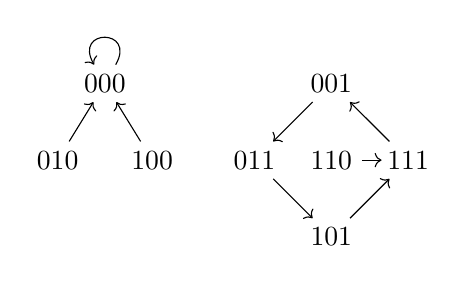
\begin{tikzpicture}[node distance=5mm and 2mm,baseline,yshift=6.1mm]
       \node (000) {$000$};
       \node[below=of 000,xshift=-6mm] (010) {$010$};
       \node[below=of 000,xshift=6mm] (100) {$100$};

       \node[right=21mm of 000] (001) {$001$};
       \node[below=of 001] (110) {$110$};
       \node[left=of 110] (011) {$011$};
       \node[right=of 110] (111) {$111$};
       \node[below=of 110] (101) {$101$};

       \draw[->] (000) to[out=60,in=120,looseness=5] (000);
       \draw[->] (001) -- (011);
       \draw[->] (010) -- (000);
       \draw[->] (011) -- (101);
       \draw[->] (100) -- (000);
       \draw[->] (101) -- (111);
       \draw[->,shorten >=-.5mm] (110) -- (111);
       \draw[->] (111) -- (001);
     \end{tikzpicture}

\end{document}